\documentclass[crop,tikz,border=5pt]{standalone}

\usetikzlibrary{fit,positioning,shapes.geometric,backgrounds,decorations.pathmorphing,decorations.markings,arrows.meta,shadows,decorations.pathreplacing}

\usepackage{libertine}          % Linux Libertine (serif)
\usepackage[libertine]{newtxmath} % Math fonts (compatible with Libertine)
\usepackage{inconsolata}        % Monospace
\usepackage[T1]{fontenc}        % Better font encoding
\usepackage{amsmath}            % Required for newtxmath

\begin{document}
  \def\pathid#1{\tikz[baseline]{\node[draw, thick, circle, anchor=base, font=\footnotesize] {#1};}}

  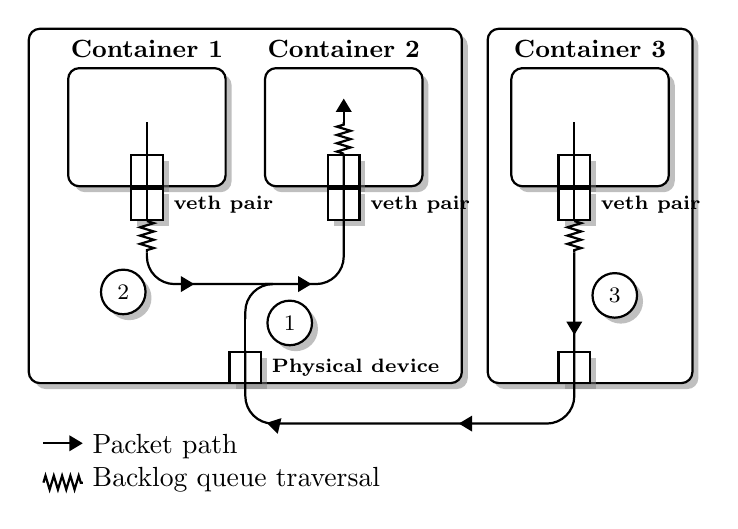
\begin{tikzpicture}[
    netns/.style={draw, thick, rounded corners, fill=white, drop shadow, minimum width=2cm, minimum height=1.5cm, align=center},
    hostns/.style={draw, thick, rounded corners, fill=white, drop shadow, minimum width=5.5cm, minimum height=4.5cm, align=center},
    device/.style={draw, thick, fill=white, drop shadow, minimum width=0.4cm, minimum height=0.4cm},
    pathid/.style={draw, thick, circle, fill=white, drop shadow, font=\footnotesize},
    pktpath/.style={thick, rounded corners=7pt},
    redirect/.style={thick, rounded corners=7pt, densely dashed, -Triangle},
    backlog/.style={thick, decorate, decoration={zigzag,segment length=3pt}}
  ]
    % Host 1 and containers 1 and 2. 
    \node[hostns] (host1) {};
    \node[netns, anchor=north west, label={[font=\small \bfseries]above:Container 1}] at ([xshift=0.5cm,yshift=-0.5cm]host1.north west) (container1) {};
    \node[netns, anchor=north east, label={[font=\small \bfseries]above:Container 2}] at ([xshift=-0.5cm,yshift=-0.5cm]host1.north east) (container2) {};
    \node[device, anchor=south] at (container1.south) (veth1) {};
    \node[device, anchor=north, label={[font=\scriptsize \bfseries]right:veth pair}] at (container1.south) (lxc1) {};
    \node[device, anchor=south] at (container2.south) (veth2) {};
    \node[device, anchor=north, label={[font=\scriptsize \bfseries]right:veth pair}] at (container2.south) (lxc2) {};
    \node[device, anchor=south, label={[font=\scriptsize \bfseries]right:Physical device}] at (host1.south) (eth1) {};

    % Host 2 and container 3.
    \node[hostns, anchor=west, minimum width=2.6cm] at ([xshift=0.3cm]host1.east) (host2) {};
    \node[netns, anchor=north, label={[font=\small \bfseries]above:Container 3}] at ([yshift=-0.5cm]host2.north) (container3) {};
    \node[device, anchor=south] at ([xshift=-0.2cm]container3.south) (veth3) {};
    \node[device, anchor=north, label={[font=\scriptsize \bfseries]right:veth pair}] at ([xshift=-0.2cm]container3.south) (lxc3) {};
    \node[device, anchor=south] at ([xshift=-0.2cm]host2.south) (eth2) {};

    % Path on same host.
    \draw[pktpath] ([yshift=0.4cm]veth1.north) -- (lxc1.south);
    \draw[backlog] (lxc1.south) -- ([yshift=-0.4cm]lxc1.south);
    \begin{scope}[decoration={markings, mark=between positions 0.2 and 0.8 step 0.35 with {\arrow{Triangle}}}]
      \draw[pktpath, rounded corners=10pt, postaction={decorate}] ([yshift=-0.4cm]lxc1.south) -- ([yshift=-0.8cm]lxc1.south) -- ([yshift=-0.8cm]lxc2.south) -- (veth2.north);
    \end{scope}
    \draw[backlog] (veth2.north) -- ([yshift=0.4cm]veth2.north);
    \draw[pktpath, -Triangle] ([yshift=0.4cm]veth2.north) -- ([yshift=0.7cm]veth2.north);

    % Path over the wire.
    \draw[pktpath] ([yshift=0.4cm]veth3.north) -- (lxc3.south);
    \draw[backlog] (lxc3.south) -- ([yshift=-0.4cm]lxc3.south);
    \begin{scope}[decoration={markings, mark=between positions 0.15 and 1 step 0.35 with {\arrow{Triangle}}}]
      \draw[pktpath, rounded corners=10pt, postaction={decorate}] ([yshift=-0.4cm]lxc3.south) |- ([yshift=-0.5cm]eth1.south) -- (eth1.north);
    \end{scope}
    \draw[pktpath] (eth1.north) -- ([yshift=0.4cm]eth1.north);
    \draw[pktpath, rounded corners=10pt] ([yshift=0.4cm]eth1.north) |- ([xshift=-1cm,yshift=-0.8cm]lxc2.south);

    % Path identifiers.
    \node[pathid] at ([xshift=0.35cm,yshift=0.35cm]eth1.north east) {1};
    \node[pathid] at ([xshift=-0.3cm,yshift=-0.9cm]lxc1.south) {2};
    \node[pathid] at ([xshift=0.3cm,yshift=0.7cm]eth2.north east) {3};

    % Legend
    \node[anchor=west, align=left] at ([xshift=0.7cm,yshift=-1cm]host1.south west) (legend) {Packet path\\Backlog queue traversal};
    \draw[pktpath, -Triangle] ([xshift=-0.5cm,yshift=0.25cm]legend.west) -- ([yshift=0.25cm]legend.west);
    \draw[backlog] ([xshift=-0.5cm,yshift=-0.25cm]legend.west) -- ([yshift=-0.25cm]legend.west);
  \end{tikzpicture}
\end{document}

% convert -density 200 -quality 90 vanilla-packet-paths.{pdf,png}
